\documentclass[]{article}
\usepackage{lmodern}
\usepackage{amssymb,amsmath}
\usepackage{ifxetex,ifluatex}
\usepackage{fixltx2e} % provides \textsubscript
\ifnum 0\ifxetex 1\fi\ifluatex 1\fi=0 % if pdftex
  \usepackage[T1]{fontenc}
  \usepackage[utf8]{inputenc}
\else % if luatex or xelatex
  \ifxetex
    \usepackage{mathspec}
  \else
    \usepackage{fontspec}
  \fi
  \defaultfontfeatures{Ligatures=TeX,Scale=MatchLowercase}
\fi
% use upquote if available, for straight quotes in verbatim environments
\IfFileExists{upquote.sty}{\usepackage{upquote}}{}
% use microtype if available
\IfFileExists{microtype.sty}{%
\usepackage{microtype}
\UseMicrotypeSet[protrusion]{basicmath} % disable protrusion for tt fonts
}{}
\usepackage[margin=1in]{geometry}
\usepackage{hyperref}
\hypersetup{unicode=true,
            pdfborder={0 0 0},
            breaklinks=true}
\urlstyle{same}  % don't use monospace font for urls
\usepackage{graphicx,grffile}
\makeatletter
\def\maxwidth{\ifdim\Gin@nat@width>\linewidth\linewidth\else\Gin@nat@width\fi}
\def\maxheight{\ifdim\Gin@nat@height>\textheight\textheight\else\Gin@nat@height\fi}
\makeatother
% Scale images if necessary, so that they will not overflow the page
% margins by default, and it is still possible to overwrite the defaults
% using explicit options in \includegraphics[width, height, ...]{}
\setkeys{Gin}{width=\maxwidth,height=\maxheight,keepaspectratio}
\IfFileExists{parskip.sty}{%
\usepackage{parskip}
}{% else
\setlength{\parindent}{0pt}
\setlength{\parskip}{6pt plus 2pt minus 1pt}
}
\setlength{\emergencystretch}{3em}  % prevent overfull lines
\providecommand{\tightlist}{%
  \setlength{\itemsep}{0pt}\setlength{\parskip}{0pt}}
\setcounter{secnumdepth}{0}
% Redefines (sub)paragraphs to behave more like sections
\ifx\paragraph\undefined\else
\let\oldparagraph\paragraph
\renewcommand{\paragraph}[1]{\oldparagraph{#1}\mbox{}}
\fi
\ifx\subparagraph\undefined\else
\let\oldsubparagraph\subparagraph
\renewcommand{\subparagraph}[1]{\oldsubparagraph{#1}\mbox{}}
\fi

%%% Use protect on footnotes to avoid problems with footnotes in titles
\let\rmarkdownfootnote\footnote%
\def\footnote{\protect\rmarkdownfootnote}

%%% Change title format to be more compact
\usepackage{titling}

% Create subtitle command for use in maketitle
\newcommand{\subtitle}[1]{
  \posttitle{
    \begin{center}\large#1\end{center}
    }
}

\setlength{\droptitle}{-2em}

  \title{}
    \pretitle{\vspace{\droptitle}}
  \posttitle{}
    \author{}
    \preauthor{}\postauthor{}
    \date{}
    \predate{}\postdate{}
  
\usepackage{float}

\begin{document}

\begin{center}

    \large \textbf{Regularisation in Random Forests}\\[12pt]

    \normalsize Bruna Wundervald$^{\ast 1}$, Katarina Domijan$^1$ and Andrew Parnell$^1$\\[12pt]
    $^1$Hamilton Institute, Maynooth University, Ireland\\ 
    $^{\ast}$Email: brunadaviesw@gmail.com\\[24pt]
    
\end{center}

\small \textbf{Abstract:} Shrinkage is still a hard task to perform in
tree-based methods. In this work, we evaluated and extended the current
methods. Our extension has demonstrated to be better than what was
proposed in Deng and Runger (2012), since we ended up with fewer
variables but still a good performance. Nevertheless, we see that the
method still has a lot of room for improvement, which defines our next
steps.

\normalsize

\subsection*{Introduction}

In real life problems, predictors can be hard or even economically
expensive to obtain. Shrinkage methods, also known as regularisation,
can make the coefficients regressions coefficients in a model to be
close or exactly equal to zero (Hastie, Tibshirani, and Friedman
(2009)), leading to variable selection. For tree-based methods, that do
not have regression coefficients to be shrunken, there is not yet a
standard regularisation procedure well established in the literature.
The main goals of this work are to understand and explore regularisation
approaches for trees and random forests, such as the one proposed in
Deng and Runger (2012). We describe the test the methods and propose an
extension to it.

\subsection*{Tree-based methods and shrinkage}

Consider a variable of interest \(Y_i \in \mathbb{R}\) and
\(\mathbf{x} = (x_{i1},\dots, x_{ip})'\) , \(1 \leq i \leq n\). A
statistical framework for non-parametric regression characterizes their
relationship as

\begin{equation}
y_i = f_0(\mathbf{x_i}) + \epsilon_i, \thinspace
\epsilon_i \stackrel{iid}\sim N(0, \sigma^2), 
\end{equation}

where \(f_0\) is an unknown regression function. A tree is a flexible
non-parametric method, based on the estimation of a series of binary
conditional splitting statements on the predictors space, that creates
rules with the form: \(x_j > x_{j,th}\), where \(x_j\) is the value of
the feature at \(j\) and \(x_{j,th}\) is the decision cut point. The
final model predicts \(Y\) with a constant \(c_m\) in each splitted
region \(R_m\). Random forests (Breiman (2001)) are an extension of
tree-based methods, combining B trees that are grown on bootstrapped
samples, but for each tree only a sample \(m \approx \sqrt p\) of the
predictors is considered for the splitting nodes. The prediction is an
average of all of the results in the training set.

An option for shrinkage in tree-based methods is presented in Deng and
Runger (2012), where the variable importance is penalized for each tree
when building a random forest. The authors also introduced the Guided
Regularized Random Forests (GRRF), that leverages the importance scores
calculated from a standard random forest model based on all the training
data. In this case, the penalization coefficient depends on the
previously obtained importance measures, that is

\begin{equation}
Gain_{R}(X_i, v) = 
\begin{cases}
\lambda_i Gain(X_i, v), i \notin F \text{ and} \\
Gain(X_i, v), i \in F, 
\end{cases}
\end{equation}

where \(\lambda_i \in (0, 1]\) is the coefficient for
\(X_i (i \in \{1,...P\})\).

In order to empirically verify the functionalities proposed in (Deng and
Runger (2012)), we tested the methods in a real gene dataset with 48910
columns and proposed an extension for it. First, we used the real gene
expression data to calculate the marginal correlations of all of the
predictors and the response. With that, we selected the ones with a
minimum of correlation to the response in the train set, for which the
cut point was determined as, for
\(\mathbf{x} = (x_{i1},\dots, x_{i48910})'\),

\begin{equation}
|corr(\mathbf{x_j}, \mathbf{y})| > 0.16, \thinspace
\text{for} \thinspace j = 1,\dots,48910.
\end{equation}

This prior selection strategy produced a subset of 2626 variables. With
this new smaller dataset, we run the GRRF model 100 times, using
\(\lambda = 0.8\) and \(\gamma = 0.9\). We add a new weighting
technique, proposed as

\begin{equation}
\label{eq:third}
\lambda_i = 
\begin{cases}
(1 - \gamma) \lambda_0 + \gamma \thinspace Imp'_{i} \thinspace\tau, \thinspace
|corr(\mathbf{x_i}, \mathbf{y})| \leq 0.5 \\
(1 - \gamma) \lambda_0 + \gamma \thinspace Imp'_{i}  \thinspace
|corr(\mathbf{x_i}, \mathbf{y})|, \thinspace
|corr(\mathbf{x_i}, \mathbf{y})| > 0.5
\end{cases}
\end{equation}

where \(|corr(\mathbf{x_i}, \mathbf{y})| \in [0,1]\) and the new
parameter \(\tau \in [0,1]\), where \(\tau\) it's not expected to be
bigger than 0.5 for regularisation. We compared the GRRF model, our
proposed extension and a model that uses the absolute values of the
marginal correlations as the weighting, as a benchmark. Results are in
Figure \ref{fig:weights}.

\begin{figure}[H]

{\centering 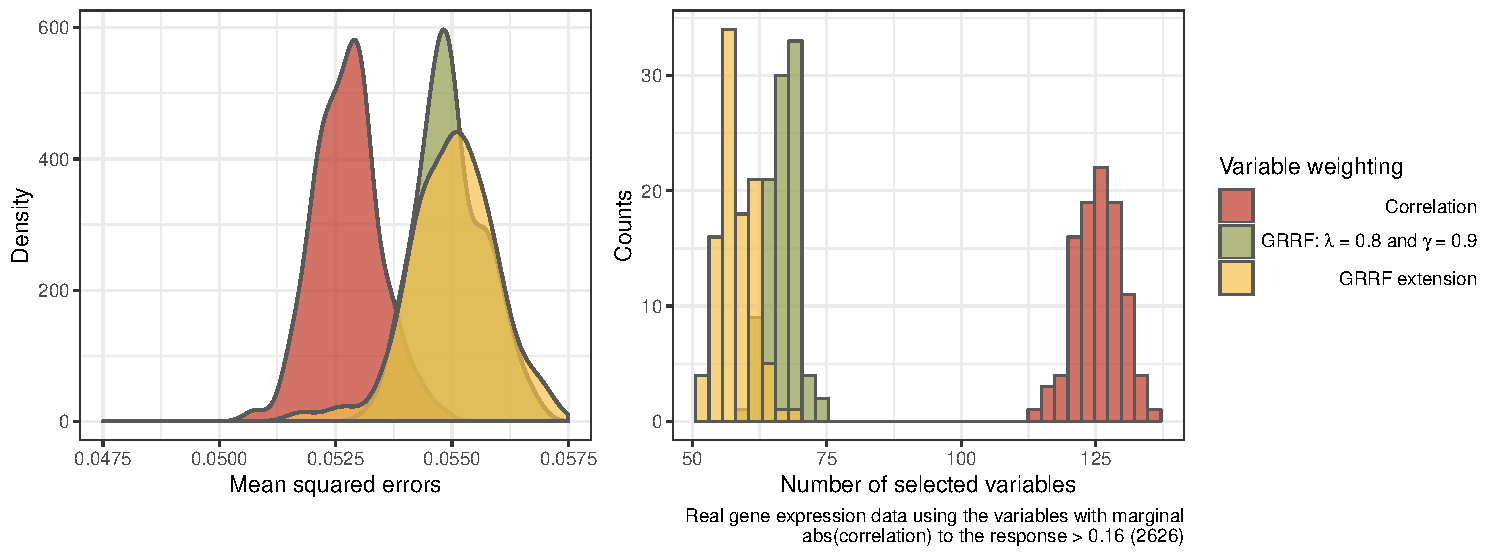
\includegraphics[width=1.1\linewidth,height=0.45\textheight]{img/weigh} 

}

\caption{Comparison of the MSR (evaluated in the test set) densities and histograms of the number of selected variables for 100 re-runs of the three models: (i) in green, the standard GRRF; (ii) in red, using simply the correlation as the variable weighting; (iii) using the methodology proposed in Equation \ref{eq:third}.}\label{fig:weights}
\end{figure}

\subsection*{Conclusions}

Shrinkage is still a hard task to perform in tree-based methods. As the
current methods do not seem to shrink enough, an extension of Deng and
Runger (2012) was proposed. In a 100 re-run of the model, our extension
presented better results, by keeping the same performance in the test
set but also having smaller numbers of selected variables, making it a
promising approach. Next steps of the project include comparing the
regularisation methods with variable selection, increasing the model
reruns, adjusting our proposed extension and improving the validation
techniques.

\subsection*{References}
\small

\hypertarget{refs}{}
\leavevmode\hypertarget{ref-Breiman2001}{}%
Breiman, Leo. 2001. ``Random Forests.'' \emph{Machine Learning}.
\url{https://doi.org/10.1017/CBO9781107415324.004}.

\leavevmode\hypertarget{ref-guided}{}%
Deng, Houtao, and George C. Runger. 2012. ``Gene Selection with Guided
Regularized Random Forest.'' \emph{CoRR} abs/1209.6425.
\url{http://arxiv.org/abs/1209.6425}.

\leavevmode\hypertarget{ref-HastieTrevor}{}%
Hastie, Trevor, Robert Tibshirani, and Jerome Friedman. 2009. ``The
Elements of Statistical Learning.'' \emph{Elements} 1: 337--87.
\url{https://doi.org/10.1007/b94608}.


\end{document}
